\chapter{线性变换}

线性变换是线性代数最常见的应用,本文将线性代数单列为一章,希望可以引起读者的重视。

在正式开始讲具体的变换之前,希望读者能从宏观上对“变换”有一个理解。我们往往将变换称为“映射”,对应的是将一个集合映射到另一个集合。函数就是一种最简单的变换。后文我们要讨论的变换也与此类似。

我们暂时先用 $\text T$ 来表示这种变换,其实矩阵乘法就是一种映射(想想为什么)。线性变换对变换本身有要求,与此前的线性运算封闭非常类似

$$
\begin{aligned}
	\text T(\mathbf u+\mathbf v) &= \text T(\mathbf u)+\text T(\mathbf v)\\
	\text T(c\mathbf u) &=c\text T(\mathbf u)
\end{aligned}
$$

\section{平移}

平移明显不是一个线性变换(想想为什么)。
平移可以直接利用向量的加法实现
$$
\text T(\mathbf w)=\mathbf w+\mathbf u_0
$$

\section{旋转}

\begin{figure}[h]
	\centering
	\includegraphics[width=0.7\linewidth]{"../img/Pasted image 20231015162403"}
	\caption{旋转矩阵的作用效果}
	\label{image_rotation}
\end{figure}

在这里不讨论旋转矩阵的具体细节,感兴趣的同学可以参考\ref{rotation_matrix}。

两个向量的点积在被旋转后保持不变。记旋转矩阵为 $\mathbf M$ 。
$$
\mathbf a^\top\cdot\mathbf b = (\mathbf M\mathbf a)^\top\cdot\mathbf M\mathbf b=\mathbf a^\top(\mathbf M^\top \mathbf M\mathbf) b 
$$
所以可得出
$$
\mathbf M\mathbf M^\top=\mathbf I 
$$



\section{投影}

投影是线性代数中很重要的一个概念,巧妙利用投影可以实现很多有意思的应用。



\subsection{投影到一条直线上}


我们先考虑将向量投影到一条直线上的情况。 $\mathbf b$ 是原向量, $\mathbf a$ 是投影的方向。 $\mathbf p$ 是投影向量。

投影的定义可以简单概括为,在 $\mathbf a$ 方向上找到一个向量 $\mathbf p$ 使其距离 $\mathbf b$ 最近。

因为 $\mathbf p$ 在$\mathbf a$ 方向上,所以 $\mathbf p$ 可以表示为 $\mathbf a \hat x$ 。$\mathbf p$ 和 $\mathbf b$ 的“距离”可以用 $\mathbf e=\mathbf b-\mathbf p$ 表示。

\begin{figure}[h]
	\centering
	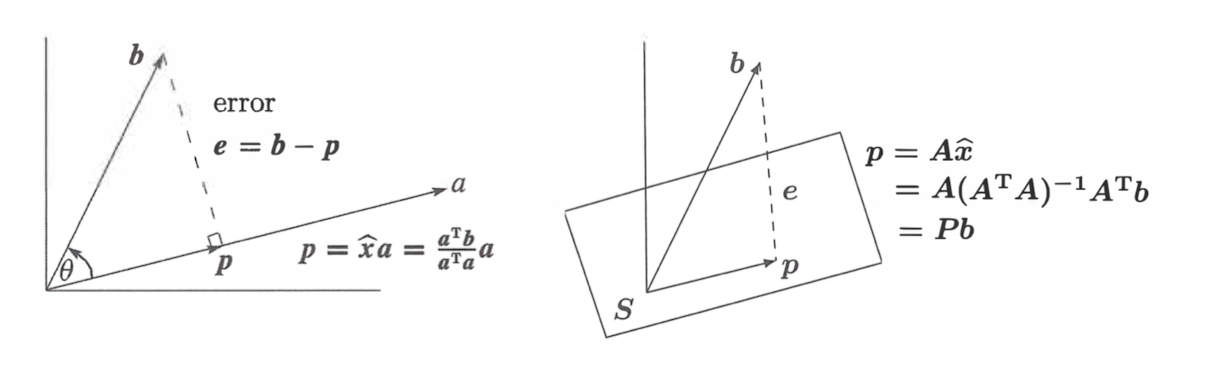
\includegraphics[width=0.7\linewidth]{../img/screenshot002}
	\caption{将 $\mathbf b$ 投影到 $\mathbf a$ 方向上}
	\label{image_line_projection}
\end{figure}

当 $\mathbf e$ 和 $\mathbf a$ 正交时这个“距离”最小。

$$
\begin{aligned}
\mathbf e\cdot\mathbf a&=0\\
(\mathbf b-\mathbf p)\cdot\mathbf a&=0\\
(\mathbf b-\mathbf a\hat x)\cdot\mathbf a&=0\\
\hat x=\frac{\mathbf a\cdot\mathbf b}{\mathbf a\cdot\mathbf a}&=\frac{\mathbf a^\top\mathbf b}{\mathbf a^\top\mathbf a}
\end{aligned}
$$

因而 $\mathbf p=\mathbf a\hat x =\mathbf a\frac{\mathbf a^\top\mathbf b}{\mathbf a^\top\mathbf a}$ ,

我们设 $P$ 为投影矩阵,可以实现将一个向量 $\mathbf b$ 投影到我们所需要的空间中,记为 $P\mathbf b$。

$$
P\mathbf b=\mathbf p=\mathbf a\frac{\mathbf a^\top\mathbf b}{\mathbf a^\top\mathbf a}
$$

故将向量投影到 $\mathbf a$ 方向的投影矩阵为 $P=\frac{\mathbf a\mathbf a^\top}{\mathbf a^\top\mathbf a}$ 。

\subsection{投影到子空间中}

问题可以转换为
\begin{quote}
	找到一个向量组合 $\mathbf p=\hat{x_1}\mathbf{a_1}+\dots+\hat{x_n}\mathbf{a_n}$ ,使得距离 $\mathbf b$ 最近。
\end{quote}

与刚才的操作类似,不同的是,所得的 $\mathbf e$ 需要与所有的 $\mathbf a_i$ 垂直。
$$
\begin{aligned}
&\mathbf {a_1}^\top(\mathbf b-A\hat{\mathbf x})=0\\
&\dots\\
&\mathbf {a_n}^\top(\mathbf b-A\hat{\mathbf x})=0
\end{aligned}
$$
写成一个矩阵的形式:
$$
\begin{aligned}
A^\top(\mathbf b-A\hat{\mathbf x})=\mathbf 0\quad& or\quad 
A^\top\mathbf b=A^\top A\hat{\mathbf x}\\
\mathbf p=A\hat{\mathbf x}&=A(A^\top A)^{-1}A^\top\mathbf b\\
\end{aligned}
$$
就可以得到投影矩阵:
$$
P=A(A^\top A)^{-1}A^\top
$$

这样的投影矩阵在工程中应用非常广泛。